\documentclass[12pt]{article}
\usepackage[utf8]{inputenc}
\usepackage[russian]{babel}
\usepackage{graphicx}
\usepackage{subcaption}
\graphicspath{ {./images/} }


\begin{document}

Дубровских Никита 221-361

\textit{\textbf{Вариант 7}}

\textit{\textbf{Задание 21.}}

\textit{Для данного графа определить, есть ли в нем эйлеров цикл и, если
есть, найти его.}

\begin{center}
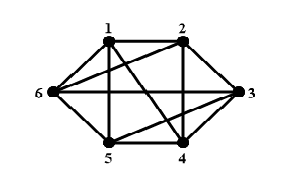
\includegraphics{21.png}
\end{center}

\underline{Решение:}

Степени всех вершин графа четные, значит эйлеров цикл есть.

Начнем строить цикл с любой вершины, например построим: 1-2-3-4-5-6-1.

Циклом охвачены все ребра.

Ответ: 1-2-3-4-5-6-1.

\end{document}
